\documentclass[letterpaper,twoside,openright,11pt,final]{memoir}

\usepackage{tipa}
\usepackage{qtree}
\usepackage{datetime}
\usepackage{terra-arcana}
\usepackage{longtable}
\usepackage{tabu}



\newcommand{\version}{150}
\newcommand{\smallimage}{100pt}
\newcommand{\audio}{{
\includegraphics[scale=0.05]{audio}}}
%%% Font setup
\newfontface\charis[Mapping=tex-text]{Doulos SIL}
\newfontfamily\mincho[Mapping=tex-text]{YuMincho}
\setmainfont[Mapping=tex-text]{Doulos SIL} 
 
%%% Custom commands 
\newcommand{\mytipa}[1]{{\charis \textipa{#1}}}
\newcommand{\bigipa}[1]{{\HUGE \charis \textipa{#1}}}

\newcommand{\blanki}{\vspace{60pt}}

%%%%% Table Separator %%%%%%
\newcommand{\tablesep}{
 &  \\
\hline
\hline
 &  \\
}

\chapterstyle{veelo}

\title{
\vspace{24pt}
\large{\textbf{Ichi, Deux, Drei!} }\\
\HUGE{Learning}\\ 
\HUGE{a new language}\\
\vfill
\large{--- RETREAT 2014 ---}
\vfill
}

\author{J.~R.~ Omahen\\
Patricia Draut}

\date{}

\begin{document}
\frontmatter

%%% Title Page
\thispagestyle{empty}
\begin{center}
\thetitle
\theauthor
\vfill
\end{center}
\newpage

%%%% Copyright page 
\thispagestyle{empty}
\ccby

\vspace{\fill}
\begin{flushleft}\normalsize

10 9 8 7 6 5 4 3 2 1 / 12 \\
\end{flushleft}

\cleardoublepage
\frontmatter
\chapter{A Brief Note}

Learning a language seems daunting, and can be unnerving for the inexperienced. Worse, the more experienced you are, the more jaded you might be -- unless you've had a particularly excellent experience. We're here to guide you on that journey. This offers a few brief looks into the most impactful areas of your study. Replete with examples, these ideas should help accelerate your learning, and give you greater success when applied consistently and diligently.

All of the examples feature audio recordings. Each item that is in a sound file is indicated by the audio icon (\audio{}). If you take the audio recordings, and add them (in order) to a playlist, you could follow this booklet from front to back.



%%%%%% Main Text %%%%%%
\mainmatter
\charis
\chapter{Vocabulary}

One of the easiest places to make big improvements is in learning new words. It may seem difficult to learn a lot of new words, but you're already good at it. I mean, look at how many words you already know! The single most common error in learning vocabulary is using your mother tongue (L1). If my mother language is English, then I should \textbf{not} use English \textbf{at all}. Instead, I should find ways around using my L1 in order to \textit{associate the thought, concept or object to the word}. After all, words are simply labels. It makes more sense to attach a label to an object, than to attach a label to an index card, with a reference of where to retrieve another label (attached to an object).

What follows are brief overviews of some of the best ways to overcome the vocabulary barrier. Even as little as 15 minutes per day will yield tremendous success over a period of time. Be consistent, and you will be rewarded.

\textit{Bonne chance!}

\section{Use Images}

The best way to overcome the L1\footnote{Your first language; mother tongue} barrier, is to use images --- \textit{visuals} --- to associate new words to the things they refer to. This can be as simple as places images next to new words, and memorising it. You can also use physical labels and place them on the objects they refer to. 

Please use the recordings to repeat the pronunciation of the word as accurately as possible.

\subsection{Hungarian}
{\huge

\begin{longtabu} to \textwidth {|X|X|}
Alma\audio{} & 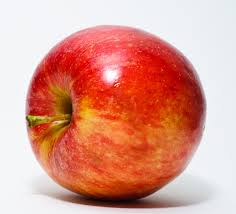
\includegraphics[width=\smallimage]{./images/alma}\\
Kenyér\audio{} & 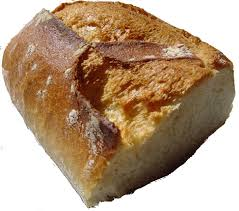
\includegraphics[width=\smallimage]{./images/kenyer}\\
Paradicsom\audio{}& 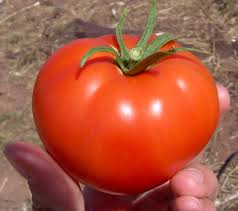
\includegraphics[width=\smallimage]{./images/paradicsom}\\
Paprika\audio{}& 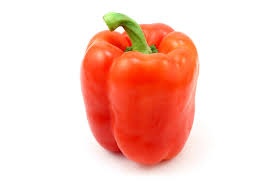
\includegraphics[width=\smallimage]{./images/paprika}\\
Zöldség\audio{}& 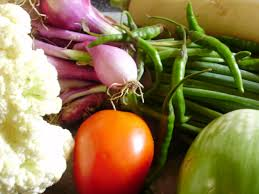
\includegraphics[width=\smallimage]{./images/zoldseg}\\
Gyümölcs\audio{}& 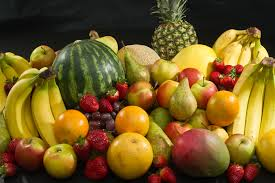
\includegraphics[width=\smallimage]{./images/gyumolcs}\\
Tej\audio{}& 
\includegraphics[width=\smallimage]{./images/tej}\\
Sajt\audio{}& 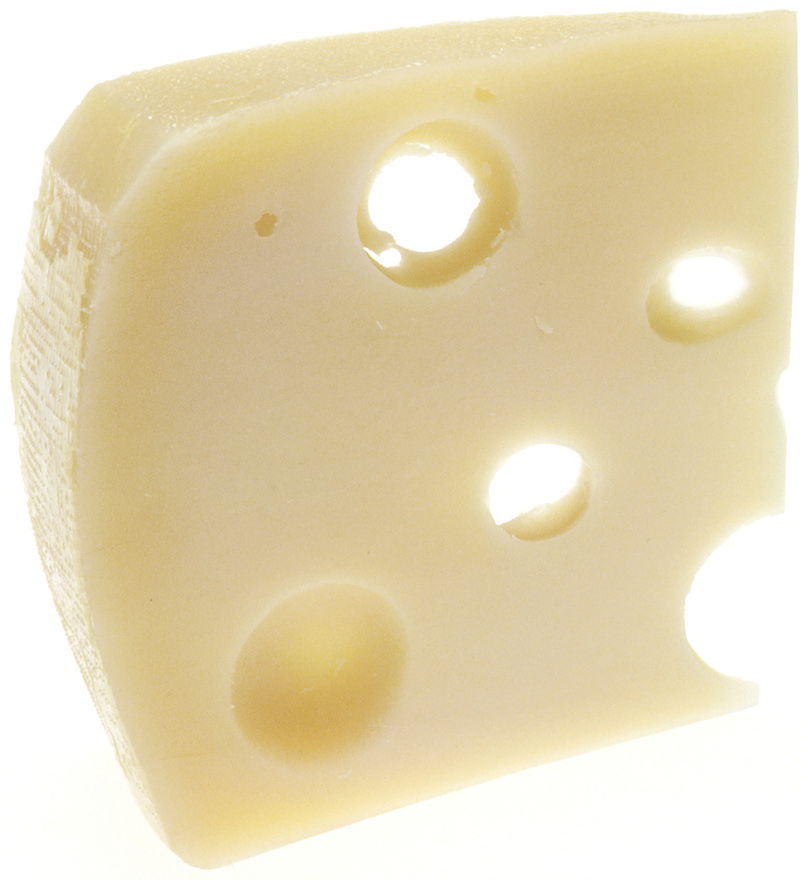
\includegraphics[width=\smallimage]{./images/sajt}\\
Hus\audio{}& 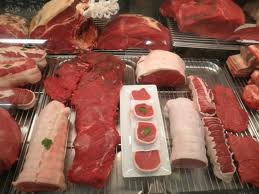
\includegraphics[width=\smallimage]{./images/hus}\\
Hal\audio{}& 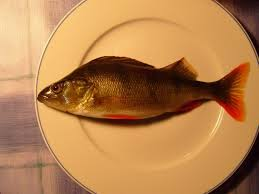
\includegraphics[width=\smallimage]{./images/hal}\\
Leves\audio{}& 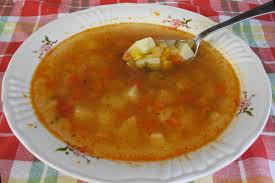
\includegraphics[width=\smallimage]{./images/leves}\\
Rizs\audio{}& 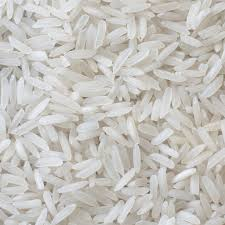
\includegraphics[width=\smallimage]{./images/rizs}\\
\end{longtabu}
}

\newpage
\subsection{Afrikaans}

For this section, you'll have to look up the words that are missing images, and draw them in yourself. In general, it's best to use a picture dictionary, or a search engine such as Google Images to avoid using your L1 if possible. In a pinch, you can look the word up in a standard dictionary, then draw an image.
{\huge
\begin{longtabu} to \textwidth {|X|X|}
'n boek\audio{}& 
\includegraphics[width=\smallimage]{./images/boek}\\
'n pen\audio{}& 
\includegraphics[width=\smallimage]{./images/stylo}\\
'n potlood\audio{}& \blanki\\
'n woordeboek\audio{}& \blanki\\
'n brief\audio{}& \blanki\\
'n bril\audio{}& \blanki\\
'n blaad\audio{}& 
\includegraphics[width=\smallimage]{./images/papier}\\
'n blaadjie\audio{}& \blanki\\
skryf\audio{}& 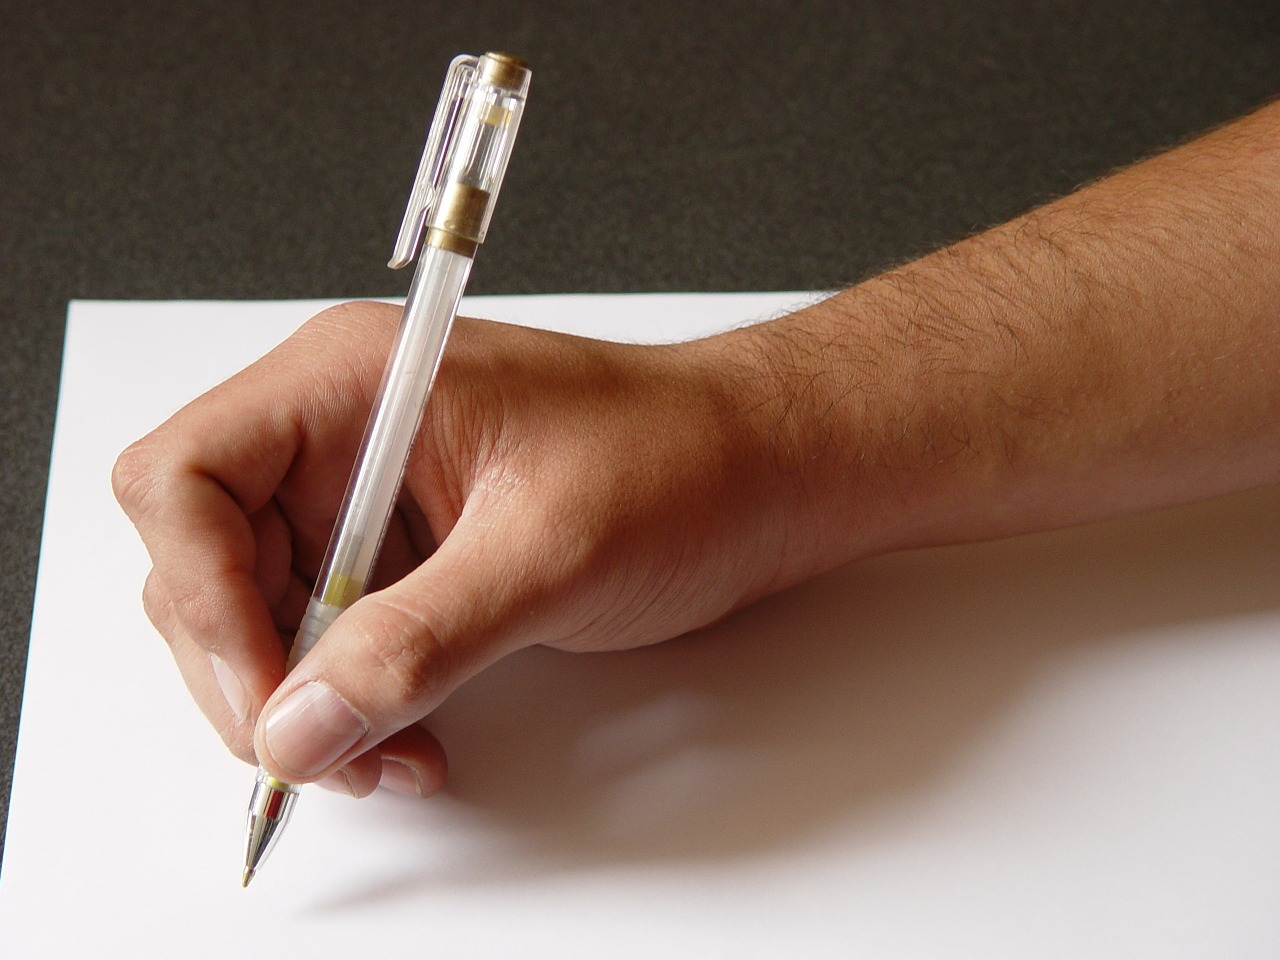
\includegraphics[width=\smallimage]{./images/skryf}\\
lees\audio{}& 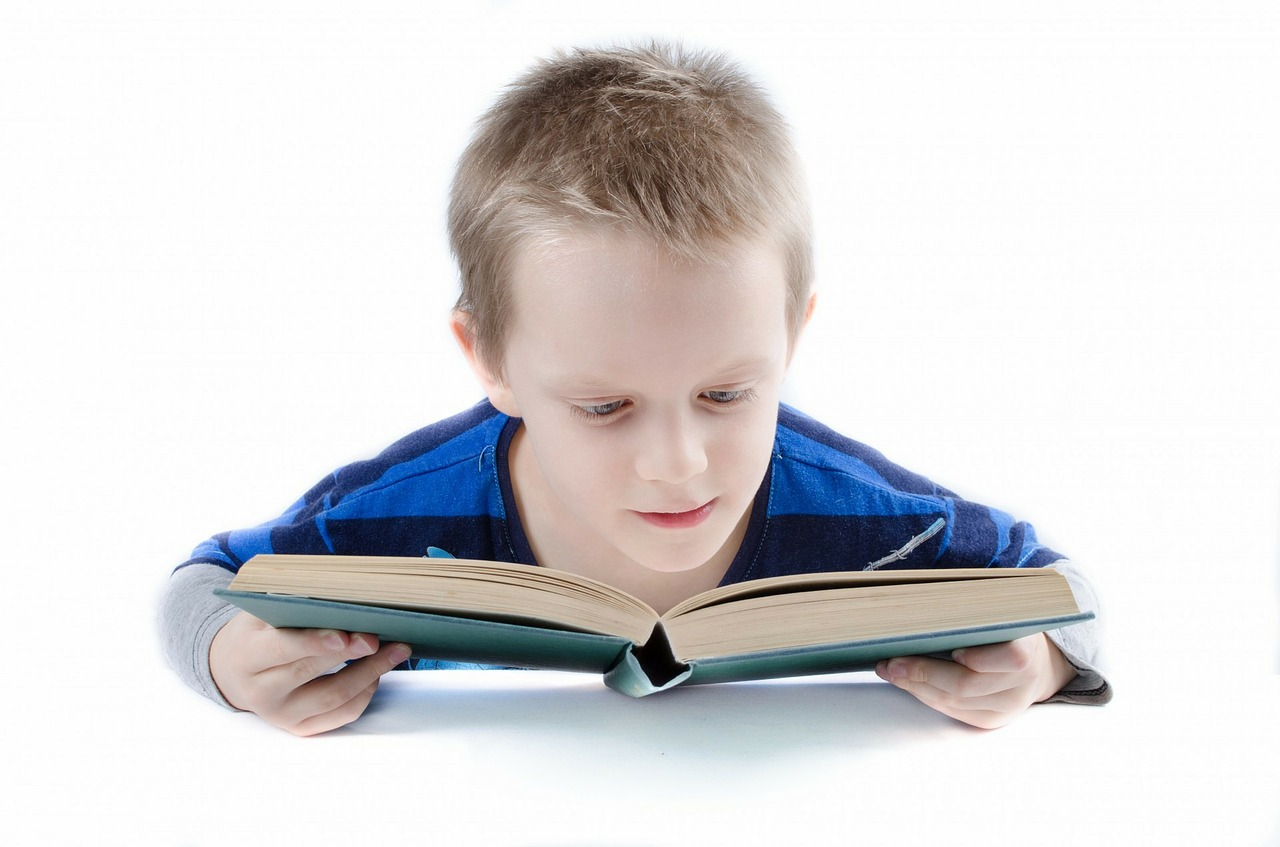
\includegraphics[width=\smallimage]{./images/lees}\\
\end{longtabu}
}

\newpage
\section{Spaced Repetition}

So how do you practically learn large amounts of words reliably in a short amount of time? The answer lies in a deceptively simple tool known as spaced repetition. Using mechanisms such as flash cards are quick and effective ways to begin committing new words to memory\footnote{\url{http://www.ncbi.nlm.nih.gov/pubmed/21988625}}. By using spaced repetition, you are strategically learning words and reviewing them on a schedule, leading to better long--term retention.

Software such as Anki\footnote{\url{http://www.ankisrs.net}} can be used effectively, as well as physical flashcards (methods such as the Leitner Box Method). However you do it, creating and testing with flash cards is exceedingly beneficial to this process. Combined with imagery, this becomes a phenomenal tool for internalising vocabulary.

\section{Semantic Domains}

Learning words randomly can be difficult. The mind doesn't jump around at random to locate where you've stored the meaning of ``tomato'', for instance. Instead, the mind works rather like a mind map: words, ideas and objects are grouped my similar meaning. You might think of the sun, for instance, and almost immediately think: sky, clouds, stars, moon. All related to the greater concept of ``things in the sky'' or ``the heavens'' or ``space''. Broadly speaking, these areas are called \textit{semantic domains}. A semantic domain is the area of meaning that words relate to. You may, for instance, think of the semantic domain of ``foods I eat for breakfast''. Learning all of these related words will be far easier for you than randomly learning 50 words, all unrelated.

Take advantage of the way your mind words and group similar ranges of meaning together, and learn groups of words faster.

\newpage
\subsection{Hungarian}
{\huge
\begin{longtabu} to \textwidth {|X|X|}
Paradicsom szelet\audio{}& 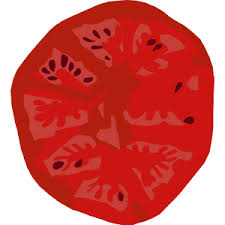
\includegraphics[width=\smallimage]{./images/paradicsomszelet}\\
Alma szelet\audio{}& 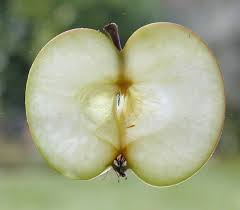
\includegraphics[width=\smallimage]{./images/almaszelet}\\
Kenyér szelet\audio{}& 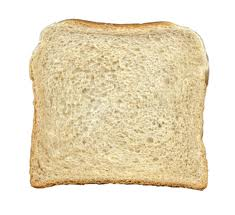
\includegraphics[width=\smallimage]{./images/kenyerszelet}\\
Paradicsom leves\audio{}& 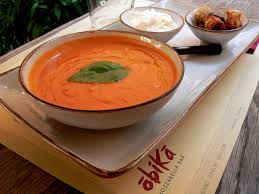
\includegraphics[width=\smallimage]{./images/paradicsomleves}\\
Gulyas leves\audio{}& 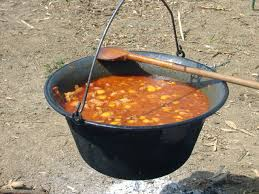
\includegraphics[width=\smallimage]{./images/gulyasleves}\\
Zöldségleves\audio{}& 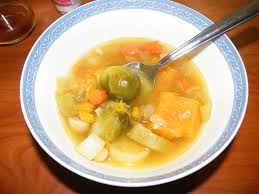
\includegraphics[width=\smallimage]{./images/zoldsegleves}\\
\end{longtabu}
}
\chapter{Grammar}

Grammar is an area that frightens most people. All grammar really means is the glue that holds words together in a meaningful fashion. It's how we create thoughts and ideas from disparate words. Depending on which L1 you're coming from, the target grammar may be easy (similar to yours) or difficult (far away from yours). The key is: you don't think consciously about the grammar you use everyday. This is the same goal you should have for your target language.

Each of these tools will help you overcome the initial hurdles of internalising grammar. Be warned: the footwork is up to you. It's not particularly difficult work, but the time you put into it will directly affect how well you learn the grammar.

\section{Use Patterns}

Especially in the beginning, most grammar can be put down to reusable patterns. Exceedingly simple sentence structure, or simple phrases are usually handled at this level. Perhaps the grammar is a little more difficult, and you need to learn noun gender? Whatever you need to learn, there will be a repeatable pattern. Inside that pattern one, maybe two, changes can occur. This is where you can substitute in words that you already know. 

The goal is to internalise grammar through patterns, using vocabulary you've already internalised. Instead of learning words and grammar, you're mostly focussed on the grammar. You won't learn in patterns forever. Down the line, when you have enough basic grammar down, you'll be able to read more complex books to learn harder grammar from.

In both of the examples below, imagine that the person speaking is holding the object (underlined vocabulary word) in front, and repeats the phrase. Imagine this person is holding each object (vocabulary word) as the sentence changes. Both of these patterns have the same meaning.\footnote{No, the meaning is not ``I am holding...'' nor ``I hold...''.}

\subsection{French}
{\huge
\begin{center}
\Tree [ [ J'ai ] [[\parbox{3em}{\underline{un}\\
  une} ] [\parbox{3em}{\underline{stylo}\\
chemise} ] ] ]
\end{center}
}
\subsection{Japanese}
{\huge
\begin{center}
\mincho
\Tree [ [ これ  は ][ \parbox{3em}{\underline{なに}?\\
                            {\large テーブル\\
                            いす \\
                            ペン}} ] ]
\end{center}
}
\charis
\section{Rinse and Repeat}

Repetition is key. But simply repeating the same terms over and over won't be beneficial. You need to repeat while changing a piece of the pattern. This internalises the overall structure, while giving you confidence and independence in choosing certain words.

\subsection{French}
{\huge
\begin{tabular}{ l | r }
J'ai & \\
 & une chemise\audio{} \\
 & une table\audio{} \\
 & une chaise\audio{} \\
 & une tasse\audio{} \\

\end{tabular}
}
\subsection{Japanese}
\mincho
{\huge
\begin{tabular}{ l | r }
これ は \underline{なに}?\audio{} & \\
 & テーブル\audio{}  \\
これ は \underline{なに}?\audio{} & \\
 & いす\audio{}  \\
これ は \underline{なに}?\audio{} & \\
 & コップ\audio{}  \\
\end{tabular}
}
\charis
\chapter{Pronunciation}

We present this section last, not due to its importance, but due to relative importance to most peolpe. We wanted to give you the answers you \textbf{really} wanted first, before hitting you with the answers \textit{to questions you didn't even think to ask}. First of all, ignore the naysayers: \textit{you can have a great accent in a new language}. It simply requires you to learn \textbf{how} and \textbf{why} speakers in your target language produce certain sounds.

If you are serious about learning a language well, it pays dividends to learn the International Phonetic Alphabet (IPA). This has been a powerful tool for linguists in analysing language, and for language learners worldwide. In learning the IPA, you will need to learn some related ideas like \textbf{voiced} and \textbf{voiceless}, \textbf{stop},\textbf{fricative}, and \textbf{affricate}. Apart from sounding really smart, you'll learn how our bodies produce the sounds of language. This gives you a powerful tool in learning how to produce new sounds that you're not used to.

In the examples below, we show you text in the native language, along with IPA. We are comparing and contrasting sounds that may be hard to master with sounds you probably know well. These kinds of conscious comparisons and exercises will greatly enhance your pronunciation and ability to hear new sounds.

\section{Practise}
\subsection{Romanian}

The key is to listen and repeat --- mimic the speaker as closely as possible. Each row highlights a sound that may be unfamiliar to you, or uncomfortable to pronounce. With daily, diligent practise, you will gain confidence and accuracy in your pronunciation.

\begin{tabu} to \textwidth {|X[l]|| X[c] X[c]}
{\Huge Ț} & preţ\audio{} & preș\audio{} \\
{\Huge /\mytipa{\t{ts}}/} & /\mytipa{"pre\t{ts}}/ & /\mytipa{"preS}/ \\
\hline
{\Huge J} & jok\audio{} & soc\audio{} \\
{\Huge /\mytipa{Z}/} & /\mytipa{"Zok}/ & /\mytipa{"sok}/ \\
\hline
\end{tabu}
\subsection{Middle Egyptian}

This pronunciation is a reconstruction, using conjectural emendation to reverse engineer the vowels from Coptic\footnote{The last phase of the Egyptian Language}, using basic vowel change extrapolation from historical records. The focus here is on two consonants that are quite difficult for English (and some other languages) speakers.

\begin{tabu} to \textwidth {|X[l]|| X[c] X[c]}
{
\includegraphics{./images/q}}\audio{} & 
\includegraphics[width=\smallimage]{./images/qala}\audio{} & 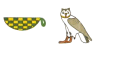
\includegraphics[width=\smallimage]{./images/kam}\audio{} \\
{\Huge /\mytipa{q}/} & /\mytipa{qa"la?}/ & /\mytipa{"kam}/ \\
\hline
{
\includegraphics{./images/c}}\audio{} & 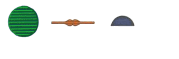
\includegraphics[width=\smallimage]{./images/casit}\audio{} & 
\includegraphics[width=\smallimage]{./images/si}\audio{} \\
{\Huge /\mytipa{C}/} & /\mytipa{Cas"it}/ & /\mytipa{"Si}/ \\
\hline
\end{tabu}

\backmatter
\chapter{\textit{Bon Voyage....}}

We wish you well on your journey! If any of these ideas interest you, or help you particularly, dig a little more in research to see how to use these ideas in other ways with more tools. Apps, worksheets, audio files, videos, flash cards and more can be found online with a small amount of research. 

If you have any questions, concerns, or just want to chat or do a Google hangout, you can reach Jonathon at \texttt{composr@gmail.com}.


\end{document}
